\section{Research method} 

\hyperref[RQ1]{RQ1} will be answered with a mapping of the field of projectional editing. 
This will follow the prescriptions of Kitchenham et al.\cite{kitchenham2015evidence}.
Gregor\cite{gregor2006nature}, gives “A Taxonomy of Theory Types in Information Systems Research”. 
To answer \hyperref[RQ2]{RQ2} and \hyperref[RQ3]{RQ3}, we will conduct what she calls “Type V: Theory for Design and Action”. 
The criteria for success of this type of research “include utility to a community of users, the novelty of the artefact, and the persuasiveness of claims that it is effective”.

We have observed the difficulty that developers have trying to reason about and edit large collections of Drools files.
We hypothesize that developers can be presented with different views on their code that will allow them to better understand the code.
The problem we wish to solve - how to improve the ability to reason about large collections of drools rules - lends itself to the technique of projectional editing.
Thus, we will apply projectional editing techniques, through the MPS language workbench to the Drools language.
The novelty of our approach will be to create new view types specific to the needs of a Drools programmer.

We will be relying on MPS as well as other open-source components to work together with acceptable performance such that the user experience is acceptable.
The reason we chose MPS is that it is the most developed of the free and open source projectional editing language workbenches, found in a study of the state of the art in Language workbenches\cite{erdweg2013state}.

Figure \ref{fig:MPS_IDE} shows the JetBrains IDE for MPS, which is also free and open-source. 
In this you create the Concepts, Generators, Type Systems, etc., that are necessary to define the language.
You also create editors, which gives your language out of the box IDE support.

\begin{figure}[!h]
    \centering
    \fbox{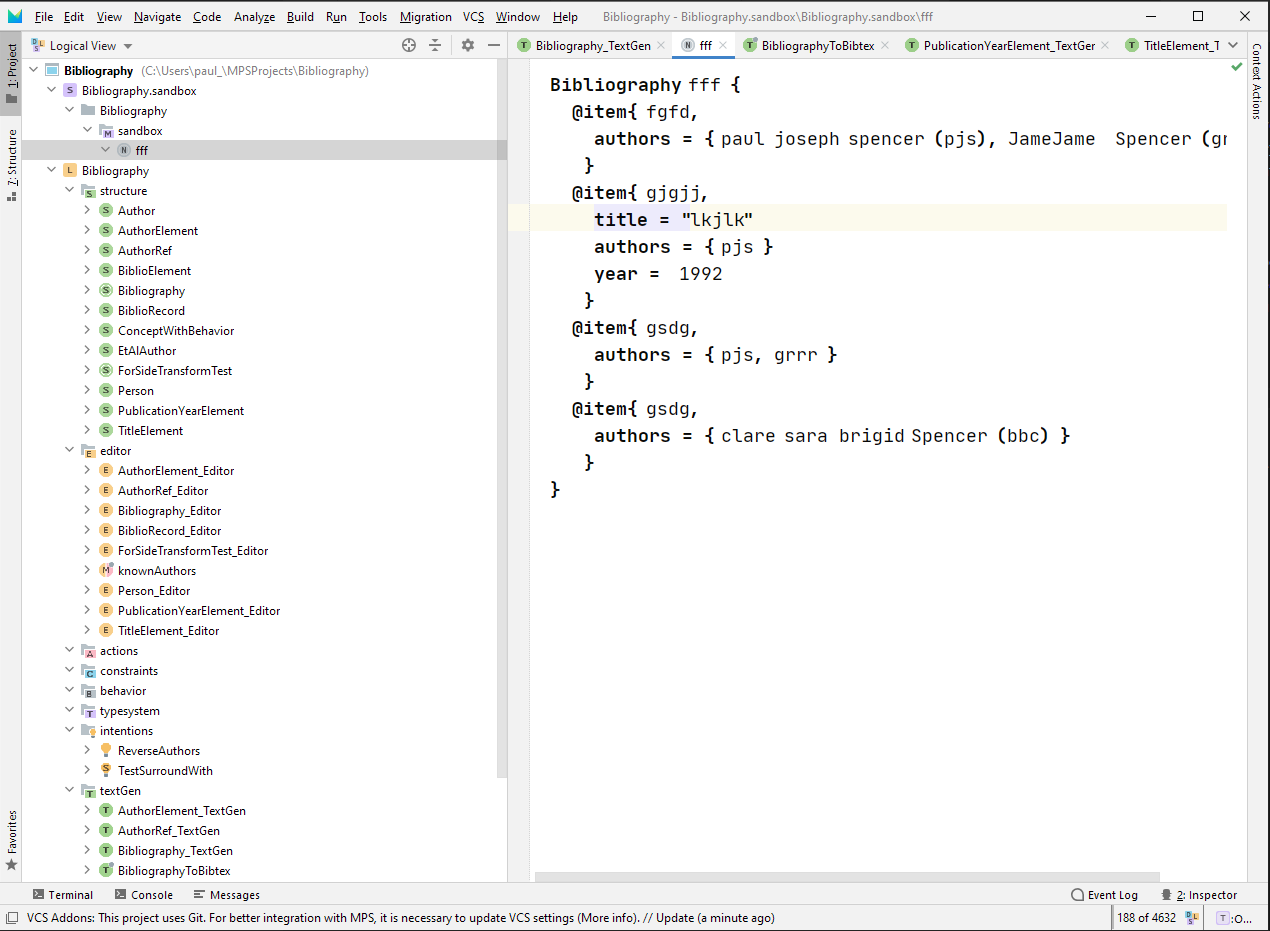
\includegraphics[width=0.95\textwidth]{images/MPS_IDE.png}}
    \caption{MPS IDE}
    \label{fig:MPS_IDE}
\end{figure}

Our designs of the projections, which will run in parallel to the Drools language modelling, will depend in part on the outcome of research carried out in the first period.
Whether our design is appropriate with regards to performance and functionality is a risk. 
Whether we can achieve usefulness in our projections also presents a risk.
This is where I expect to gain the biggest benefit of literature review and academic supervision. 

The prototype will consist of a base of the Drools language, re-defined in MPS.  
On top of this will be a set of different projections of the AST.
Whilst we have not decided on the projections yet, some examples may include:
\begin{itemize}
    \item Visualization of order of execution.
    \item Spreadsheet-like decision tables.
    \item "Group-by" fact, query or function usage.
\end{itemize}


The major tasks in this prototype development will be: 
\begin{itemize}
    \item Modelling the Drools language.
    \item Developing the alternative projections.
\end{itemize}

The prototype itself will be validated by working and being novel.
However, if time permits, the hypothesis of the usefulness of the projections will be validated through developer use surveys.

